\section{Rolamento; Momento Angular}
\subsection{Conteúdo Importante}
\subsubsection{Rolamento sem Escorregamento}

Quando um corpo rígido simétrico redondo (e.g. uma esfera ou um cilíndro uniforme) de raio $R$ rola sem escorregar sob uma superfície horizontal, a distância percorrida pelo seu centro (quando as suas rodas rodam por um ângulo $\theta$) é igual ao comprimento do arco pelo qual um ponto na extremidade se move:

\begin{equation}
    \Delta x_{CM}=s=R\theta
\end{equation}

\begin{figure}[h!]
    \centering
    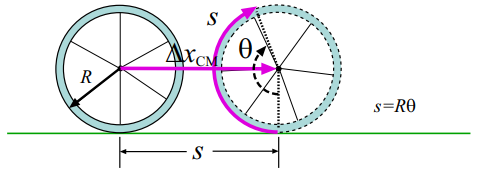
\includegraphics[width=0.5\textwidth]{8/fig/rolSemEscor.png}
    \caption{Ilustração da relação entre $\Delta x$, $s$, $R$ e $\theta$ para um objeto em rolamento.}
\end{figure}

A velocidade do centro de massa para o objeto em rolamento, $v_{CM}=\frac{dx_{CM}}{dt}$ e a sua velocidade angular estão relacionados por

\begin{equation}
    v_{CM}=R\omega
\end{equation}

e a magnitude da aceleração do centro de massa está relacionado com a aceleração angular por:

\begin{equation}
    a_{CM}=R\alpha
\end{equation}

A energia cinética do objeto é:

\begin{equation}
    K_{rolamento}=\frac{1}{2}I_{CM}\omega^2+\frac{1}{2}Mv^2_{CM}
\end{equation}

O primeiro termo à direita representa a energia cinética rotacional do objeto sob o seu eixo de simetria; o second termo representa a energia cinética que o objeto teria se se movesse com velocidade $v_{CM}$ sem rolar. No fundo, $K_{rol}=K_{rot}+K_{trans}$.

Quando uma roda rola sem escorregar, \emph{pode} haver força de atrito a agir na superfície da mesma. Neste caso, é uma força de atrito \emph{estático} e dependendo da situação, poderá ter a mesma direção ou oposta ao movimento do centro de massa.

\subsubsection{Torque como Vetor}
No último capítulo, foi dada uma definição para a torque $\tau$ que atua num corpo rígido em rotação sobre um eixo fixo. Agora, é dada uma definição mais geral para "torque"; a "torque" é definida atuando numa única partícula quando uma força atua sobre a mesma.

Supondo que o vetor posição (relativo à origem $O$) de uma partícula é $r$ e uma única força $F$ atua sobre ela. Então, a torque $\tau$ atuando na partícula é

\begin{equation}
    \tau=r\times F
\end{equation}

Se $\phi$ for o ângulo entre o vetor posição $r$ e a força $F$, então a torque $\tau$ tem magnitude

\begin{equation*}
    \tau=rF\sin\phi
\end{equation*}

\subsubsection{Momento Angular de Uma Partícula e de Sistema de Partículas}
Se uma partícula tem um vetor posição $r$ e momento linear $p$, ambos relativos a uma origem $O$, então o \textbf{momento angular} dessa partícula (relativo à origem) é definido por:

\begin{equation}
    L=r\times p=m(r\times v)
\end{equation}

O momento angular tem unidades $kg\cdot m^2\cdot s^{-1}$.
É possível mostrar que a torque resultante numa partícula é igual à derivada em ordem ao tempo do momento angular:

\begin{equation}
    \sum \tau=\frac{dL}{dt}
\end{equation}

Para um conjunto de pontos de massa em movimento, o momento angular total é definido como a soma vetorial dos momentos angulares individuais:

\begin{equation*}
    L=L_1+L_2+L_3+...
\end{equation*}

A taxa à qual o momento angular total muda está relacionado com as torques que surgem de forças exceridas fora do sistema.

\begin{equation}
    \sum \tau_{ext}=\frac{dL}{dt}
\end{equation}

Isto diz-nos que quandoi a soma das torques externas é zero, então \textbf{L} é constante (conservado).

\subsubsection{Momento Angular para Rotação sobre Eixo Fixo}
Para uma rotação sobre um eixo fixo, o "momento angular" do objeto rígido é um número, $L$. Além disso, é possível mostrar que se a avelocidade angular do objeto for $\omega$ e o seu momento de inércia sobre o eixo dado é $I$, então o seu momento angular sobre o eixo é

\begin{equation}
    L=I\omega
\end{equation}

\subsubsection{Conservação do Momento Angular}
Para um sistema no qual não há torque externa resultante, o momento angular total mantém-se constante: $L_i=L_f$. Este princípio é conhecido como a \textbf{Conservação do Momento Angular}.